\subsection{Doppelspaltversuche mit Elektronen}
\label{subsec:doppelspalt_elektronen}

Der Wellencharakter des Elektrons\index{Wellencharakter!des Elektrons} wird
besonders deutlich im Doppelspaltversuch\index{Doppelspaltversuch}. Dieser
Versuch ist eines der wichtigsten Experimente der Quantenmechanik
\index{Quantenmechanik}, weil er zeigt, dass Elektronen weder vollständig wie
klassische Teilchen noch vollständig wie klassische Wellen beschrieben werden
können.

Beim klassischen Doppelspaltversuch mit Licht\index{Licht} entsteht auf einem
Schirm ein Interferenzmuster\index{Interferenzmuster}. Lichtwellen, die durch
zwei Spalte laufen, überlagern sich. An manchen Stellen verstärken sie sich,
an anderen löschen sie sich teilweise aus. Dadurch entstehen helle und dunkle
Streifen.

Führt man einen entsprechenden Versuch mit Elektronen\index{Elektron} durch,
erwartet man aus klassischer Sicht zunächst ein anderes Ergebnis. Wären
Elektronen nur kleine geladene Teilchen\index{Teilchen}, dann müssten sie
entweder durch den linken oder durch den rechten Spalt fliegen. Auf dem Schirm
würden dann im Wesentlichen zwei Auftreffbereiche entstehen, ähnlich wie bei
kleinen Kügelchen.

Das tatsächliche Ergebnis ist jedoch anders. Auch Elektronen erzeugen ein
Interferenzmuster. Besonders bemerkenswert ist dies, wenn die Elektronen einzeln
durch die Versuchsanordnung geschickt werden. Jedes Elektron wird auf dem Schirm
als einzelner Punkt registriert. Nach vielen Elektronen entsteht aus diesen
einzelnen Punkten jedoch wieder ein Interferenzmuster.
\FloatBarrier
\begin{figure}[H]
	\centering
	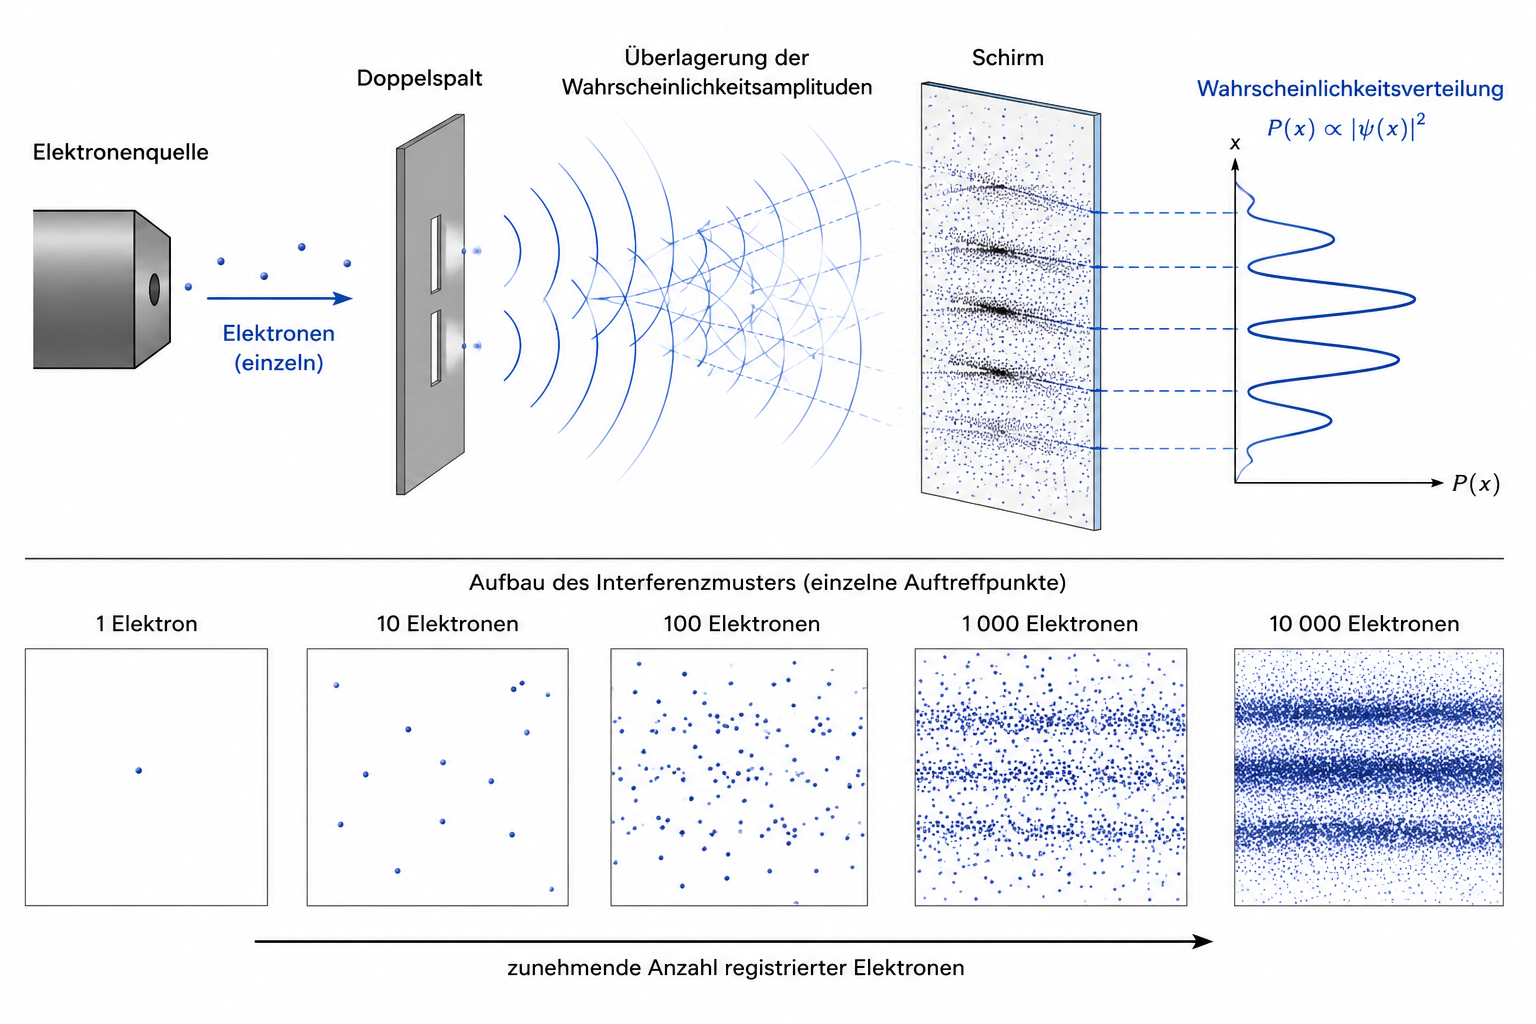
\includegraphics[width=0.85\textwidth]{bilder/doppelspaltversuch}
	\caption{Schematische Darstellung des Doppelspaltversuchs mit Elektronen. 
		Einzelne Elektronen werden punktförmig auf dem Schirm registriert. Nach vielen 
		Elektronen entsteht ein Interferenzmuster, das den Wellencharakter der 
		quantenmechanischen Wahrscheinlichkeitsverteilung zeigt.}
	\label{fig:doppelspalt_elektronen}
\end{figure}


Damit zeigt der Versuch zwei Seiten des Elektrons. Die Registrierung auf dem
Schirm erfolgt punktförmig. In diesem Sinn erscheint das Elektron als Teilchen.
Die Verteilung vieler Auftreffpunkte folgt jedoch einem Interferenzmuster. In
diesem Sinn zeigt das Elektron Welleneigenschaften\index{Welleneigenschaft}.

\begin{PhysicsBox}[Elektronen im Doppelspaltversuch]
	\label{box:elektronen_doppelspalt}
	Ein einzelnes Elektron wird punktförmig gemessen. Viele einzeln gemessene
	Elektronen bilden jedoch ein Interferenzmuster. Das Muster zeigt den
	Wellencharakter der quantenmechanischen Wahrscheinlichkeitsverteilung.
\end{PhysicsBox}

Entscheidend ist dabei nicht, dass ein Elektron eine klassische Welle wäre. Es
breitet sich nicht wie eine Wasserwelle als sichtbare Materieverteilung aus.
Stattdessen beschreibt die Quantenmechanik\index{Quantenmechanik} den Zustand
des Elektrons durch eine Wellenfunktion\index{Wellenfunktion}. Aus dieser
Wellenfunktion ergibt sich eine Wahrscheinlichkeitsverteilung
\index{Wahrscheinlichkeitsverteilung} für mögliche Auftrefforte auf dem Schirm.

Mathematisch wird diese Wahrscheinlichkeit durch den Betrag der Wellenfunktion
beschrieben:

\begin{equation}
	P(\vec r) \propto |\psi(\vec r)|^2
	\label{eq:wahrscheinlichkeit_wellenfunktion}
\end{equation}

Dabei ist \(\psi(\vec r)\)\index{Wellenfunktion} die Wellenfunktion des
Elektrons und \(P(\vec r)\)\index{Wahrscheinlichkeit} die Wahrscheinlichkeit,
das Elektron am Ort \(\vec r\) zu finden. Das Interferenzmuster entsteht also
nicht aus einer klassischen Bahn des Elektrons, sondern aus der Überlagerung
von Wahrscheinlichkeitsamplituden\index{Wahrscheinlichkeitsamplitude}.

Versucht man festzustellen, durch welchen Spalt das Elektron gegangen ist,
verschwindet das Interferenzmuster. Die Messung\index{Messung} verändert die
Situation grundlegend. Sobald die Weginformation\index{Weginformation}
verfügbar ist, verhält sich die Verteilung der Elektronen nicht mehr wie ein
Interferenzbild, sondern eher wie die Verteilung klassischer Teilchen.
Ein Elektron besitzt im Doppelspaltversuch keine klassische Bahn, solange keine
Weginformation gewonnen wird.
Der Doppelspaltversuch mit Elektronen zeigt damit den Kern der Quantenmechanik:

Die Theorie liefert stattdessen Wahrscheinlichkeiten für Messergebnisse. Erst
bei der Messung wird ein bestimmter Auftreffpunkt registriert.

Diese Erkenntnis ist für das Verständnis des Atoms entscheidend. Auch im Atom
bewegt sich das Elektron nicht auf einer festen Kreisbahn um den Kern. Es wird
durch eine Wellenfunktion beschrieben. Aus dieser Wellenfunktion entstehen
später die Orbitale\index{Orbital}, also räumliche
Wahrscheinlichkeitsverteilungen für den Aufenthaltsort des Elektrons.